\begin{comment}
\end{comment}

\chapter{Construction de codes correcteurs quantiques}
\label{chap:construction_codes}

Dans le chapitre précédent, 
je me suis intéressé à la correction des erreurs lors de la communication classique.
Pour la suite de la thèse,
je quitterai ce régime pour m'intéresser au régime quantique.
Dans ce chapitre, 
j'aborderai plus particulièrement à la protection de l'information 
dans un modèle de bruit quantique simplifié avant de présenter la conception d'une mémoire 
quantique au prochain chapitre.
Ce modèle simplifié ressemble au canal binaire symétrique présenté au premier chapitre
et il permet d'étudier la construction de codes correcteurs d'erreurs quantiques sans prendre en compte les détails d'implémentation.

De façon semblable au scénario classique,
concevoir des codes correcteurs qui permettent de bien protéger l'information avec un nombre raisonnable de qubits supplémentaires est crucial.
En fait,
la présence des erreurs est l'un des obstacles parmi les plus
limitants pour la réalisation de calculs quantiques.
Ainsi, 
la correction d'erreurs ne se limite pas à des scénarios de communication 
comme dans le cas classique,
mais sera omniprésente dans un système de calcul quantique.

Cette importance accrue des erreurs dans les systèmes quantiques s'explique
principalement du fait qu'il s'agit de systèmes analogues plutôt que digitaux.
Un système est digital lorsque chacun de ses éléments peut prendre un nombre fini
de valeurs. 
Dans le cas des ordinateurs classiques,
chaque bit prend soit la valeur 0 ou la valeur 1.
Ainsi,
une quantité continue comme une différence de potentiel représente physiquement un bit tout en le protégeant des erreurs.
Par exemple,
le bit 0 peut être associé à une valeur de 0 volt et le bit 1 à une valeur de 5 volts.
Dans le cas où une valeur de 4.9 volts serait mesurée, il est fort probable que 
la valeur désirée était le bit 1.
Donc, en absence des perturbations externes présentes lors de la communication,
l'information classique est relativement robuste.

Au contraire, un système quantique est analogue puisqu'il existe une infinité d'états accessibles.
Par exemple, toutes paires de nombres complexes $a$ et $b$ telles que $|a|^2 + |b|^2 = 1$
représentent l'état d'un qubit.
Ainsi, 
une faible variation de ces paramètres engendre un état différent
et distinguer l'état désiré d'un état corrompu est généralement impossible.
De plus, l'accumulation de ces petites différences peut complètement
changer le résultat d'un calcul.

Ces erreurs émergent généralement de processus de décohérence.
Par exemple,
un système quantique dans un état excité tend naturellement à retourner dans un état de moindre énergie.
Au milieu des années 1990,
plusieurs scientifiques croyaient que
les erreurs engendrées par la décohérence des systèmes quantiques
représentaient un obstacle insurmontable au calcul quantique~\cite{unruh_maintaining_1995, palma_quantum_1996, landauer_is_1995, chuang_quantum_1995}.
Leurs arguments reposaient entre autres sur le théorème de non-clonage~\cite{wootters_single_1982}
stipulant qu'il est impossible de copier l'état d'un qubit vers un second qubit.
Cela semblait donc empêcher l'utilisation de la redondance pour 
protéger le système des erreurs comme c'est le cas pour la communication classique.

Nous savons aujourd'hui comment contourner ces limitations. 
Les premiers à avoir proposé une solution sont Calderbank, Shor et Steane~\cite{calderbank_good_1996, steane_multiple-particle_nodate}.
D'ailleurs, à la prochaine section,
je vais introduire une importante famille de codes correcteurs quantiques, les codes CSS, qui portent leur nom.
En réponse à ce résultat, Gottesman~\cite{gottesman_stabilizer_1997} a introduit le formalisme des codes stabilisateurs
que je vais utiliser dans ce chapitre pour décrire les codes correcteurs quantiques.

Depuis,
plusieurs familles de codes correcteurs quantiques ont été introduites.
Les codes les plus étudiés sont sans aucun doute les codes de surfaces et 
les codes toriques introduits par Kitaev~\cite{kitaev_fault-tolerant_2003}.
Cependant,
ces codes, bien qu'excellents pour protéger le système,
ne permettent pas d'encoder efficacement un grand nombre de qubits~\cite{bravyi_tradeoffs_2010}.
Pour contrer ce problème,
les codes quantiques d'opérateurs de parité à faible 
densité~(LDPC, de l'anglais \textit{low-density parity-check})
reçoivent de plus en plus d'attention.
Cet intérêt est en partie stimulé par le succès des codes LDPC classiques introduits
par Gallager~\cite{gallager_low-density_1962}.
De plus, il a été montré par Gottesman~\cite{gottesman_fault-tolerant_2013}
qu'il est possible d'utiliser des codes quantiques LDPC pour 
construire des ordinateurs quantiques protégés des erreurs avec 
un surcout constant en qubits.
Il s'agit donc d'outils importants pour la réalisation du calcul quantique à grande échelle.

Les codes quantiques LDPC incluent plusieurs familles,
dont les codes par produit d'hypergraphes~\cite{tillich_quantum_2014}
et les codes par produit homologique~\cite{bravyi_homological_2014}.
Comme l'indique le nom de ces exemples,
les codes quantiques LDPC sont généralement obtenus par le produit 
de structures associées à des codes correcteurs classiques.
Dans le cadre de cette thèse,
j'ai conçu une approche qui permet plutôt de générer des codes correcteurs quantiques
directement,
sans avoir recours à une construction classique au préalable.
L'un des principaux avantages de cette méthode est sa flexibilité 
lors de la construction des codes.
En fait,
cette construction permet théoriquement de générer n'importe quelle famille de codes stabilisateurs,
dont les codes LDPC.
De plus,
les résultats des expériences numériques suggèrent que de nombreuses famille de codes peuvent 
être générées efficacement avec cette approche.

Cette approche repose sur la résolution d'un problème de satisfaction de contraintes,
un problème fondamental et très étudié de l'informatique classique~\cite{lecoutre_constraint_2009}.
Bien que ce problème soit généralement difficile à résoudre,
j'ai numériquement identifié des régimes pour lesquels il est aisé de
construire des codes correcteurs quantiques
et des régimes pour lesquels la tâche est beaucoup plus ardue.
Cela, bien que surprenant, est un comportement attendu pour ce type de problème.

Je reviendrai sur cela après avoir présenté le formalisme des canaux bruités quantiques 
et des codes stabilisateurs.
Finalement,
je présenterai l'article expliquant la construction et 
mettant de l'avant les résultats de ce projet.

\section{Correction d'erreurs quantique}

\subsection{Canaux bruités quantiques}

Un état quantique est généralement représenté par un opérateur de densité $\rho$
de trace unité.
Une évolution arbitraire d'un état $\rho$ vers un état $\rho'$
c'est-à-dire une combinaison d'opérations unitaires,
de mesures et d'interactions avec l'environnement, 
est représentée par une application
\begin{align}
  \rho' = \mathcal{E}(\rho).
\end{align}
Pour décrire plus précisément cette transformation,
j'utiliserai les opérateurs de Krauss.
Dans ce cas,
l'application est définie par
\begin{align}
  \mathcal{E}(\rho) = \sum_{k} E_k \rho E_k^\dag,
\end{align}
avec la condition que 
\begin{align}
  \sum_k E_k^\dag E_k = I.
\end{align}
Cette dernière permet d'assurer que $\tr(\mathcal{E}(\rho)) = 1$.

Dans leur excellent livre d'introduction à l'informatique quantique, 
Neilsen et Chuang~\cite{nielsen_quantum_2010} motivent en détail 
cette définition générale pour l'évolution d'un état quantique.
Ainsi, je me limite à une justification intuitive de cette définition
et j'invite les personnes intéressées à consulter le huitième chapitre de ce livre.

De façon générale,
l'état $\rho$ évolue au sein d'un environnement dont les états de base 
sont $\qty{\ket{e_0}, \ket{e_1}, \ldots}$.
Sans perte de généralité,
le système et l'environnement sont supposés dans un état de produit tensoriel,
soit un état sans intrication.
Aussi, il est suffisant de considérer que l'environnement est dans l'état 
pur $\ket{e_0}$.
Ainsi,
l'état initial du système et de l'environnement est $\rho \otimes \op{e_0}$.

\begin{figure}
  \begin{center}
    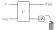
\includegraphics{figures/circuit_canal_quantique.pdf}
  \end{center}
  \caption[Représentation en circuit d'un canal quantique]{
    Représentation en circuit d'un canal quantique.
    Le résultat de la mesure est ignoré.
  }
  \label{fig:circuit_canal_quantique}
\end{figure}

Par la suite,
un opérateur unitaire $U$ est appliqué sur le système et l'environnement,
suivi d'une mesure de l'environnement sans connaitre le résultat.
Le circuit correspondant est illustré à la figure~\ref{fig:circuit_canal_quantique}.
Ainsi, l'état final du système est
\begin{equation}
  \mathcal{E}(\rho) 
  = \tr_{\text{env}}\qty(U(\rho \otimes \op{e_0})U^\dag)
  = \sum_k \bra{e_k}U(\rho \otimes \op{e_0}) U^\dag \ket{e_k}
  = \sum_k E_k \rho E_k^\dag
\end{equation}
avec $E_k = \mel{e_k}{U}{e_0}$.
Alors,
l'application $\mathcal{E}$ représente la transformation de l'état d'un système quantique
lorsque celui-ci interagit avec son environnement alors qu'on ignore l'état final
de l'environnement.

Une autre interprétation est qu'à la suite de l'application $\mathcal E$,
le système se retrouve dans l'état $\rho_k \propto E_k \rho E_k^\dag$
avec probabilité $p_k = \tr(E_k \rho E_k^\dag)$.
Il est alors possible d'écrire l'application selon
\begin{align}
  \mathcal E(\rho) = \sum_k p_k \rho_k.
\end{align}
Cette formulation montre clairement l'utilité de $\mathcal E$ pour
représenter un canal bruité quantique.
De façon comparable au canal bruité classique,
un canal quantique transforme un premier état 
vers un second état choisi aléatoirement.

Dans cette thèse,
je me limite aux canaux bruités quantiques avec des opérateurs 
de Krauss $E_k$ proportionnels aux opérateurs de Pauli.
Les opérateurs de Pauli pour un seul qubit sont 
\begin{align}
  &I = \op{0}{0} + \op{1}{1}, 
  &&Y = -i\op{0}{1} + i\op{1}{0}, \notag \\
  &X = \op{0}{1} + \op{1}{0}, 
  &&Z = \op{0}{0} - \op{1}{1}.
\end{align}
Le groupe~\footnote{Je fais un rappel des notions de théorie des groupes à l'annexe~\ref{chap:theo_groupes}}
de Pauli $\mathcal P_n$ de $n$ qubits est un groupe multiplicatif sur 
l'ensemble des opérateurs $\qty{I, X, Y, Z}^n$ avec une phase parmi $\qty{1, i, -1, -i}$.
Dans ce cas,
le canal s'écrit généralement comme
\begin{align}
  \mathcal E(\rho) = \sum_{P \in \mathcal P_n} p_P P\rho P.
\end{align}
Le poids $|P|$ d'un opérateur de Pauli $P$ est le nombre d'opérateurs différents de $I$ qui le composent.
Par exemple, $|i\cdot XIYX| = 3$.
Pour l'ensemble des canaux que je considèrerai,
la probabilité d'une erreur $P \in \mathcal P_n$ diminue exponentiellement avec le poids 
de celle-ci.

De prime abord,
cette approche semble limitée,
mais puisque les opérateurs de Pauli forment une base,
il est possible de représenter un opérateur de Krauss
comme une combinaison linéaire de ces derniers.
Ainsi,
un protocole qui permet de protéger un système quantique contre les erreurs 
$Q \subseteq \mathcal P_n$ protège également le système contre toutes les 
combinaisons linéaires des opérateurs de $Q$~\cite{knill_theory_1997}.
Ce modèle est donc suffisant pour construire une théorie générale de la correction d'erreurs quantique.

En particulier,
dans l'article de ce chapitre,
j'utilise le canal d'effacement quantique pour évaluer la performance
des codes correcteurs que je construis.
Ce canal représente la situation où l'information contenue dans certains qubits
est complètement perdue et qu'il est possible d'identifier ces qubits.
On dit alors que ces qubits sont effacés.
En laboratoire, cela correspond par exemple à la défaillance d'une composante électronique
ou à la perte d'un photon.
Pour représenter cette situation, l'état $\rho$ est associé à un second registre
permettant de marquer les qubits effacés.
Dans le cas d'un seul qubit avec une probabilité d'effacement $p$,
le canal s'écrit
\begin{equation}
  \mathcal E_p(\rho \times \op{0}) 
  = (1 - p) \rho \otimes \op{0} + p \frac{I}{2} \otimes \op{1}.
\end{equation}
Dans cette équation,
l'opérateur $I/2$ est utilisé pour représenter un état complètement mixte
sans aucune information sur l'état initial $\rho$.
Le second registre indique la présence de l'effacement.
Comme 
\begin{align}
  I = \frac{1}{2} \qty(
  I\rho I + X \rho X + Y \rho Y + Z \rho Z
)
\end{align}
pour tout opérateur $\rho$\footnote{
  En notant $f(\rho) = I\rho I + X\rho X + Y \rho Y + Z \rho Z$,
  on remarque que $f(I/2) = 2I$ et que $f(X) = f(Y) = f(Z) = 0$.
  De plus,
  pour avoir une trace unité,
  une matrice densité se décompose comme $\rho = I/2 + aX + bY + cZ$,
  ce qui permet de conclure.
},
il est possible de réécrire le canal à l'aide d'opérateurs de Pauli à deux qubits.
Ainsi,
\begin{equation}
  \mathcal E_p(\rho \times \op{0}) 
  = \qty(1 -  p) \rho \otimes \op{0} + \frac{p}{4} \qty(\rho + X \rho X + Y \rho Y + Z \rho Z)\otimes \qty(X\op{0}X).
\end{equation}

Dans l'article,
je présente plus en détail le canal d'effacement.
Entre autres,
je généralise le canal au cas à plusieurs qubits
en plus de présenter un algorithme de décodage optimal applicable à n'importe quel
code correcteur quantique pour ce canal.
Ce décodeur universel est la raison principale pour utiliser le canal d'effacement.
Celui-ci permet d'étudier de nouveaux codes sans nécessairement avoir besoin de construire des 
décodeurs spécialisés pour des canaux bruités plus complexes~(voir par exemple \cite{pastawski_holographic_2015, gullans_quantum_2021}).

Dans le chapitre suivant,
j'utiliserai un modèle de bruit plus réaliste qui permet
de représenter une mémoire quantique.
Celui-ci est également construit à partir d'opérateurs de Krauss proportionnels à des
opérateurs de Pauli.

\subsection{Codes stabilisateurs}
\label{sec:codes_stabs}

L'une des meilleures ressources pour une présentation complète du formalisme des codes
stabilisateurs est la thèse de doctorat de Gottesman~\cite{gottesman_stabilizer_1997}.
Dans cette section,
je me limiterai plutôt aux concepts essentiels à la compréhension des travaux et de l'article.

De façon comparable aux codes classiques,
les codes correcteurs quantiques encodent les états d'un espace de Hilbert
dans un sous-espace d'un espace de plus grande dimension.
Dans le cas des qubits,
les états de l'espace de Hilbert $\mathcal H_2^k$ sont encodés à l'aide d'un
sous-espace $\code \subseteq \mathcal H_2^n$.
Ainsi,
si $\ket\psi, \ket\phi \in \code$,
alors $\alpha\ket\psi + \beta\ket\phi \in \code$ 
pour toutes paires $\alpha, \beta$ de nombres complexes.~\footnote{
  Pour simplifier la présentation,
  je laisse tomber la normalisation des états quantiques.
}

Un exemple de code quantique permettant d'encoder un qubit à l'aide de neuf qubits est 
le code de Shor~\cite{shor_scheme_1995} défini par l'encodage
\begin{align}
  \ket{0} \to \ket{\bar{0}} = (\ket{000} + \ket{111}) \otimes (\ket{000} + \ket{111}) \otimes (\ket{000} + \ket{111}), \notag \\
  \ket{1} \to \ket{\bar{1}} = (\ket{000} - \ket{111}) \otimes (\ket{000} - \ket{111}) \otimes (\ket{000} - \ket{111}).
  \label{eq:code_shor}
\end{align}
Par linéarité, l'état $\alpha \ket{0} + \beta \ket{1}$ est encodé avec l'état 
$\alpha \ket{\bar{0}} + \beta\ket{\bar {1}}$.
Je ne détaillerai pas ce code,
mais celui-ci illustre qu'il n'est pas pratique d'énumérer l'encodage des états de base
pour définir un code.
D'abord,
l'espace $\mathcal H_2^k$ requiert $2^k$ états de base
et chacun de ceux-ci implique une superposition de $\mathcal O(2^n)$ états
si le code $\code$ est un sous-espace de l'espace de Hilbert à $n$ qubits.

Le formalisme des stabilisateurs permet de contourner ce problème en offrant une 
représentation beaucoup plus efficiente de certains états quantiques.
D'abord,
un état $\ket\phi$ est stabilisé par l'opérateur $U$ lorsque $U\ket\psi = \ket\psi$,
soit lorsque $\ket \phi$ est un état propre de valeur propre $+1$ de $U$.
Un état ou un sous-espace est alors représenté par les opérateurs qui le stabilisent.
Par exemple,
l'état $\ket{00} + \ket{11}$ est l'unique état à deux qubits stabilisé par 
les opérateurs $XX$ et $ZZ$. 
De même,
les états $\ket{00}$ et $\ket{11}$ forment une base
pour les états stabilisés par l'opérateur $ZZ$.
Il est important de choisir des opérateurs qui commutent pour s'assurer 
que ceux-ci partagent les mêmes états propres.
De plus, l'opérateur identité $I$ stabilise tous les états
et l'opérateur $-I$ ne stabilise aucun état.

De façon plus générale,
un groupe stabilisateur $\mathcal S$ pour $n$ qubits est un sous-groupe abélien 
du groupe de Pauli $\mathcal P_n$ excluant l'opérateur $-I$.
Cette exclusion implique également que tous les opérateurs ayant la phase $i$ ou $-i$ sont exclus.
Un code stabilisateur $\code(\mathcal S)$ est alors l'espace des états stabilisés par $\mathcal S$.
De plus,
puisque les états stabilisés par les opérateurs $P, Q \in \mathcal P_n$ sont également
stabilisés par l'opérateur $PQ$,
il est commun de choisir un ensemble de générateurs $g(\mathcal S) = \qty{S_1, \ldots, S_m}$
pour décrire le groupe stabilisateur
\begin{align}
  \mathcal S = 
  \qty{
    \prod_{i=1}^m S_i^{a_i} : \vb a \in \qty{0, 1}^m
  }
\end{align}
de $2^m$ éléments.
Lorsque les générateurs sont indépendants,
c'est-à-dire qu'il n'est pas possible d'en obtenir un comme le produit des autres,
le code $\code(\mathcal S)$ a une dimension $2^{n - m}$.
Ainsi, 
pour encoder $k$ qubits avec un code de $n$ qubits,
exactement $m = n - k$ générateurs indépendants sont nécessaires.

Le code de Shor introduit à l'équation~\eqref{eq:code_shor} est stabilisé
par le groupe généré par les opérateurs 
\begin{gather}
    X_1 X_2 X_3 X_4 X_5 X_6, \quad
    Z_1 Z_2, \quad Z_4 Z_5, \quad Z_7 Z_8, \notag \\
    X_4 X_5 X_6 X_7 X_8 X_9, \quad
    Z_2 Z_3, \quad Z_5 Z_6, \quad Z_8 Z_9.
\end{gather}
Dans ce cas précis,
le formalisme stabilisateur peut sembler légèrement encombrant,
mais il permet généralement de représenter un code de $n$ qubits encodant $k$ qubits
à l'aide de $n - k$ opérateurs de poids $\mathcal O(n)$.
Le cout total de la représentation est alors $\mathcal O(n^2)$, ce qui est un gain exponentiel
par rapport à l'énumération des états de base du code en notation de Dirac.
Pour la suite,
j'utiliserai la notation $[n, k]$ pour représenter un code stabilisateur arbitraire 
encodant l'espace $\mathcal H_2^k$ dans un sous-ensemble $\code \subseteq \mathcal H_2^n$.

Le syndrome d'une erreur $E \in \mathcal P_n$,
qui affecte un état $\ket\psi$ quelconque d'un code $[n, k]$,
est le résultat des mesures des générateurs du groupe stabilisateur.
Puisque les opérateurs de Pauli commutent ou anticommutent,
le résultat de chacune de ces mesures est $+1$ ou $-1$.
En effet, si $SE = \pm ES$ pour un stabilisateur $S$,
alors
\begin{equation}
  SE\ket\psi = \pm E S \ket\psi = \pm E\ket\psi.
\end{equation}
Ainsi,
l'état $E\ket\psi$ est un état propre de valeur propre $\pm 1$ de $S$.
Les composantes du syndrome $\vb{s}(E) \in \qty{+1, -1}^{n - k}$
sont données par la relation $S_iE = s_i S_i E$ pour $S_i \in g(\mathcal S)$.

Il est important de noter que le syndrome est indépendant de l'état $\ket \psi$.
Conséquemment,
une mesure du syndrome permet de détecter la présence d'erreurs sans corrompre l'état du système.
À partir de cette information,
un décodeur essaie de trouver une correction $F$ telle que $FE \in \mathcal S$, 
soit une correction telle que $FE\ket\psi = \ket\psi$ pour tout état code $\ket\psi$.
Le choix de la correction n'est pas unique, car, si $FE \in \mathcal S$,
alors $(SF)E \in \mathcal S$ pour tous $S \in \mathcal S$.
Ainsi,
toutes corrections $F' = SF$ sont équivalentes.

Formellement,
tous les opérateurs $P \in \mathcal P_n$ de la même classe du groupe quotient $\mathcal P_n/\mathcal S$
ont le même effet sur le code puisque $P\ket\psi = PS\ket\psi$ pour tout $S \in \mathcal S$.
La classe d'un opérateur $P \in \mathcal P_n$ est l'ensemble $P\cdot \mathcal S = \qty{PS : S\in \mathcal S}$,
soit l'ensemble des opérateurs équivalents après multiplication par un stabilisateur.
De plus,
comme $|\mathcal P_n| = 4^{n+1}$,
le groupe quotient $\mathcal P_n/\mathcal S$ d'un code $[n, k]$ tel que $|\mathcal S| = 2^{n - k}$
possède $2^{n+k+2}$ classes.
En comparaison,
seulement $2^{n-k}$ syndromes sont possibles,
ce qui implique que $2^{2k + 2} = 4^{k + 1}$ classes d'opérateurs ont exactement le même syndrome,
mais des effets différents sur le code.

Les opérateurs appartenant aux classes ayant le syndrome $\qty{+1, +1, \ldots, +1}$
sont des représentations à $n$ qubit des opérateurs de Pauli $\mathcal P_k$
agissant sur le code~\cite{aaronson_improved_2004}.
Ces opérateurs forment le groupe des opérateurs logiques $\mathcal L$ et correspondent
au centralisateur~\footnote{
  Il est en réalité nécessaire de considérer le normalisateur du groupe stabilisateur,
  mais pour un sous-groupe du groupe de Pauli,
  le centralisateur et le normalisateur sont égaux.
  J'utilise donc le centralisateur directement pour simplifier la présentation.
},
\begin{align}
  \qty{P \in \mathcal P_n : PS = SP, \forall S \in \mathcal S},
\end{align}
du groupe stabilisateur.
Puisqu'un opérateur logique $L \in \mathcal L$ commute avec l'ensemble des stabilisateurs,
\begin{equation}
  S(L\ket\psi) = LS\ket\psi = L\ket\psi
\end{equation}
pour tout état code.
En conséquence,
$L\ket\psi$ est également un état code.
De façon similaire,
pour un syndrome arbitraire,
les $4^{k+1}$ classes ayant ce syndrome sont reliées par les opérateurs logiques.

On remarque que $\mathcal S \subset \mathcal L$.
En effet, le groupe stabilisateur correspond à l'opérateur $I$ sur le code.
De même, les classes $-\mathcal S$, $i\mathcal S$ et $-i\mathcal S$ correspondent
aux opérateurs $-I$, $iI$ et $-iI$.
La correspondance entre les autres opérateurs logiques et opérateurs de Pauli est
arbitraire tant que les relations de commutation sont respectées.

La conséquence de tout cela est qu'il est possible de décomposer un opérateur
$E \in \mathcal P_n$ en produit $LT$ où $T$ est un opérateur de même syndrome que $E$
et $L$ est un opérateur logique.
Il n'est pas nécessaire que $E = LT$, mais plutôt que $LT$ soit un élément de la classe $E \cdot \mathcal S$.
Cette décomposition permet de construire une procédure de décodage optimale que l'on 
nomme décodeur par maximum de vraisemblance (MV).
À partir du syndrome de l'opérateur $E$, 
le décodeur MV choisi d'abord aléatoirement une correction $T$ de même syndrome avant
de choisir un opérateur logique selon
\begin{align}
  L_{\text{MV}} = \arg\max_{L \in \mathcal L} \sum_{S \in \mathcal S} \Pr[LST].
\end{align}
L'idée derrière le décodeur MV est qu'il existe un opérateur logique $L^*$ tel que $T = L^*E$.
Alors, le décodage est un succès si $L_{MV}$ et $L^*$ ont la même classe,
c'est-à-dire si $L_{MV}T = SE$ pour un certain stabilisateur $S \in \mathcal S$.
Ainsi, pour tout opérateur logique $L$, nous avons que 
\begin{align}
  \sum_{S\in \mathcal S} \Pr[LST]
  =
  \sum_{S\in \mathcal S} \Pr[LSL^*E]
  =
  \sum_{S\in \mathcal S} \Pr[LL^*SE].
\end{align}
Dans le cas typique,
le poids de $E$ est faible puisque la probabilité d'un opérateur diminue avec son poids.
Ainsi, la somme est maximisée par $LL^* \in \mathcal S$ si le poids de chacun des opérateurs de
$\mathcal L \setminus \mathcal S$ est élevé.
Sinon,
la somme est maximisée par $LL^* \equiv P \in \mathcal L \setminus \mathcal S$ 
et l'application de cette correction laisse le système avec une erreur $L_{MV}TE = LL^*EE = P$ indédectable.

Le décodeur échoue dans deux cas,
soit si le poids de $E$ est élevé, ce qui est hors de notre contrôle,
ou s'il existe un opérateur logique non stabilisateur de faible poids.
Ainsi,
il est important de construire des codes stabilisateurs pour lesquels la distance minimale,
\begin{align}
  d = \min_{L \in \mathcal L \setminus \mathcal S} |L|,
\end{align}
est élevée.
Le décodeur MV permet de corriger toutes les erreurs dont le poids est inférieur à $d / 2$.
Il n'est pas exclu que des erreurs de poids plus élevé soit corrigibles, 
mais les paramètres $n$, $k$ et $d$ d'un code permettent d'estimer rapidement la capacité
de ce dernier à corriger les erreurs en fonction de son rendement $k/n$.
Par exemple,
la distance minimale du code de Shor est trois.
Ainsi, ce code permet de corriger toutes les erreurs de poids un.
Dans le cas où la probabilité d'une erreur de poids $w$ est proportionnelle $p^w$,
le code de Shor réduit la probabilité d'erreur logique d'un facteur quadratique.

Par contre,
calculer la distance minimale d'un code requiert de comparer le poids d'un nombre exponentiel d'opérateurs.
Il en est de même pour le calcul de $L_{MV}$ qui requiert généralement un nombre exponentiel de comparaisons.
Une des exceptions à ce grand cout pour le décodeur MV est pour le canal à effacement pour lequel
le cout est  polynomial.
Ainsi, dans les travaux de cette thèse,
j'ai effectué des simulations numériques du canal à effacement avec le décodeur MV pour estimer la
capacité des codes que j'ai construits.
Les codes étudiés dans l'article appartiennent 
à la famille des codes CSS que je présente à la prochaine section.

\subsection{Codes CSS}

Un opérateur est de type $P$ pour $P \in {X, Y, Z}$ s'il est un produit tensoriel de $I$ et $P$ exclusivement.
Les codes de Calderbank-Shor-Steane (CSS)~\cite{calderbank_good_1996, steane_multiple-particle_nodate},
sont des codes stabilisateurs générés par un ensemble composé uniquement d'opérateurs de type $X$ et $Z$.
Le code de Shor de l'équation~\ref{eq:code_shor} est un exemple de code CSS.
L'avantage des codes CSS provient du fait qu'il est possible de décomposer n'importe quelle opérateur
de Pauli comme un produit d'un opérateur de type $X$ et d'un opérateur de type $Z$.
Ainsi,
la partie $X$ d'une erreur sera détectée par les générateurs de type $Z$ et vice-versa.
Cela permet alors de simplifier l'analyse et les décodeurs en séparant le traitement des générateurs 
et des erreurs de chaque type.
Les générateurs $g(\mathcal S)$ du groupe stabilisateur $\mathcal S$
code CSS sont donc partitionnés en deux sous-ensembles $g_X(\mathcal S)$ et $g_Z(\mathcal S)$,
où $g_P(\mathcal S)$ contient les générateurs de type $P$.

Construire un code CSS, et par extension un code stabilisateur, n'est pas simple,
puisque les stabilisateurs doivent commuter.
Pour vérifier si deux opérateurs de Pauli commutent ou anticommutent,
il est suffisant de vérifier la commutation sur chaque qubit individuellement.
En effet,
deux opérateurs parmi $\qty{I, X, Y, Z}$ agissant sur le même qubit commutent si l'un d'entre 
eux est trivial ($I$) ou s'ils sont égaux.
Sinon, ils anticommutent.
Conséquemment,
deux opérateurs à plusieurs qubits commute si et seulement si ils anticommutent sur un nombre 
pair de qubits.
Pour les codes CSS, 
un opérateur de type $X$ commute avec un opérateur de type $Z$ si le nombre de qubits où les deux
agissent non-trivialement est pair.

Bien évidemment,
la théorie des codes CSS est beaucoup plus riche que ce que je viens de présenter.
Cependant,
les relations de commutations entre les opérateurs sont suffisantes pour comprendre
les travaux présentés à la fin de ce chapitre.
Je reviendrai plus en détail sur les codes CSS au prochain chapitre lorsque je présenterai
la construction des codes par produit d'hypergraphes.
 
\subsection{Représentations des codes stabilisateurs}
\label{sec:representations_codes}

La méthode de construction de codes présentée dans l'article de chapitre est en fait un algorithme
de recherche d'ensembles d'opérateurs de Pauli qui commutent.
Pour définir ce problème,
j'utilise deux représentations alternatives des codes, à savoir les matrices de parités et les graphes de Tanner.
Par simplicité,
je limiterai ses représentations aux codes CSS,
mais il est possible de les généraliser à tous les codes stabilisateurs.

Un opérateur de Pauli à $n$ qubits de type $P$ s'exprime comme $\otimes_{i=1}^{n} P^{p_i}$,
où $\vb p \in \corpsfini{2}^{n}$ est ce que l'on nomme un opérateur de parité.
Dans cette représentation,
une paire d'opérateurs de Pauli de type $X$ et $Z$ ayant respectivement les opérateurs de parité $\vb x$ 
et $\vb z$ commutent si $\vb x^T \vb z = 0$,
soit lorsque $\vb x$ et $\vb z$ sont orthogonaux.
Comme un stabilisateur peut être représenté par un opérateur de parité,
il est possible de représenter les générateurs $g_P(\mathcal S)$ d'un code CSS
par une matrice $H_P$ dont la rangée $i$ est l'opérateur de parité du
générateur $S_{P, i}$.
Les matrices $H_X$ et $H_Z$ sont les matrices de parité du code.
Ces dernières doivent respecter la condition $H_X^t H_Z = 0$ pour 
que les stabilisateurs commutent.

Un code est éparse si le nombre de 1 dans chacune des matrices est faible.
Formellement,
une famille de codes est éparse si le ratio entre le nombre de 1 
et le nombre total d'éléments de ces matrices de parité tend vers zéro 
lorsque la taille du code augmente.
Les codes éparses sont également nommés codes LDPC,
de l'anglais \textit{Low-Density Parity-Check} se traduisant par
\textit{opérateurs de parité à faible densité}.
Comme je le présenterai à la section suivante,
les codes LDPC sont particulièrement importants puisqu'il est possible de construire
des circuits de mesure du syndrome avec un faible surcout
constant en nombre de qubits~\cite{gottesman_fault-tolerant_2013}.
Ainsi,
ces circuits de faible taille limitent la propagation des erreurs en plus d'être plus simple à 
implémenter en laboratoire.
Un point fort de la méthode présentée dans l'article de ce chapitre est qu'elle permet 
de générer de tels codes.

Les matrices de parité permettent également d'obtenir une représentation graphique d'un code.
Pour ce faire, la matrice de parité $H_P$ est associée à la matrice d'adjacence d'un
graphe biparti $T_P = (Q \cup g_P(\mathcal S), A_P)$,
où $Q = \qty{q_1, \dots, q_n}$ est l'ensemble des qubits
et $\qty{q_i, S_{P, j}} \in A_P$ si et seulement si $H_{P, i, j} = 1$.
Les graphes $T_X$ et $T_Z$ sont les graphes de Tanner de $g_X(\mathcal S)$ et $g_Z(\mathcal S)$.
Il est possible de combiner ces deux graphes en un seul graphe
\begin{align}
  T = (Q \cup g(\mathcal S), A_X \cup A_Z)
\end{align}
pour obtenir le graphe de Tanner de $g(\mathcal S) = g_X(\mathcal S) \cup g_Z(\mathcal S)$.
La première figure de l'article de ce chapitre illustre le graphe de Tanner du code de Shor.

D'un point de vue haut niveau,
la méthode de construction de codes présentée dans cette thèse
débute avec un graphe biparti ayant un nombre important d'arête.
Ensuite, elle cherche un graphe de Tanner comme sous-graphe de ce graphe.
Cette recherche est analogue à un problème de coloration des arêtes du graphe initiale.
On dit alors qu'un graphe admet un coloriage stabilisant s'il possède un graphe de Tanner comme sous-graphe.

Les problèmes de coloriage de graphes figurent parmi les problèmes de satisfaction de contraintes.
Ainsi,
il est possible de construire des codes stabilisateurs en utilisant les méthodes 
de résolutions des problèmes de statisfaction de contraintes.
Je définirai ces problèmes à la section suivante.

\section{Problèmes de satisfaction de contraintes}
\label{sec:csp}

Les problèmes de satisfaction de contraintes (PSC)
forment l'une des classes de problèmes parmi les plus importantes en informatique.
Un exemple de PSC est le problème de coloriage d'une carte illustré à la figure~\ref{fig:quebec}.
Dans ce cas,
il s'agit d'assigner une couleur à chacune des régions d'une carte sans que deux régions voisines 
aient la même couleur.
Pour représenter ce problème,
il est courant d'utiliser un graphe où les sommets représentent les régions et une arête relie
chaque paire de régions voisines.
Ceci n'est qu'un des nombreux exemples de PSC.
Ces derniers trouvent de nombreuses applications dans plusieurs domaines,
dont l'intelligence artificielle~\cite{russel_artificial_nodate}
et la compilation de langages de programmation~\cite{aho_compilers_2006}.

\begin{figure}
  \begin{center}
    \includegraphics{figures/quebec.pdf}
  \end{center}
  \caption[Exemple du problème de coloriage d'une carte]{
    Carte des régions administratives du Québec et exemple de coloriage. 
    Le coloriage utilise quatre couleurs,
    ce qui est optimal puisque le graphe contient un sous-graphe complet
    formé par les quatre sommets 6, 13, 14 et 15~\cite{kubale_graph_2004}.
    Image modifiée à partir de Wikimedia Commons~\cite{noauthor_carte_2016}.
  }
  \label{fig:quebec}
\end{figure}

De façon générale,
un PSC est défini par trois ensembles~\cite{lecoutre_constraint_2009},
soit un ensemble de variables $V = \qty{v_1, \ldots, v_n}$,
un ensemble de domaines $D = \qty{d_1, \ldots, d_n}$
et un ensemble de contraintes $C = \qty{c_1, \ldots, c_m}$.
Chaque variable $v_i$ prend les valeurs du domaine $d_i$
et chaque contrainte $c_j$ est une paire $(T_j, R_j)$
telle que $T_j$ est un sous-ensemble ordonné de variables et $R_j$
est un sous-ensemble du produit des domaines correspondants.
Une assignation $a: V \to D$ satisfait une contrainte $(T, R)$ 
si $(a(v) : v \in T) \in R$.
Un PSC est satisfiable s'il existe une assignation 
satisfaisant toutes les contraintes simultanément.

Pour le coloriage d'un graphe $G = (S, A)$,
les variables correspondent aux sommets $S$
et le domaine de chaque variable est le même,
soit les couleurs disponibles.
Une contrainte $(a, D^*)$ est ajoutée pour chaque arête $a \in A$,
où $D^*$ est l'ensemble des paires de couleurs différentes.
Une assignation satisfait l'ensemble des contraintes 
si chaque paire de sommets d'une même arête a deux couleurs différentes.
Pour l'exemple de la figure~\ref{fig:quebec},
le problème est satisfiable si et seulement si quatre couleurs 
ou plus sont disponibles ~\cite{kubale_graph_2004}.

La méthode de construction de codes proposée est une variation 
du coloriage d'un graphe biparti où les couleurs sont assignées aux arêtes plutôt qu'aux sommets.
Dans ce cas, il y a une couleur pour chaque opérateur de Pauli $\qty{I, X, Y, Z}$
et les contraintes assurent que le coloriage correspond à un graphe de Tanner
en plus d'assurer d'autres propriétés favorables à la découverte de meilleurs codes.

Ce problème est généralement difficile à résoudre,
mais comme pour plusieurs autres PSC difficiles,
les résultats numériques que j'ai obtenus suggèrent fortement
l'existence d'un régime de paramètres pour lesquels la recherche d'assignations
satisfaisant les contraintes est beaucoup plus facile.
De plus,
les logiciels de résolutions des PSC sont de plus en plus efficients comme le démontrent les résultats
de diverses compétitions du domaine~\cite{noauthor_minizinc_nodate, noauthor_sat_nodate}.
Ce sont ces deux raisons qui me portent à croire que la connexion entre la construction de 
codes stabilisateurs et les problèmes de satisfaction de contraintes a le potentiel de grandement accélérer la découverte de codes correcteurs quantiques.

À la prochaine section, 
je présente un PSC pour lequel l'existence de différents régimes de difficulté 
est bien étudiée. 
De plus, je présente une motivation théorique un peu plus générale pour l'existence de
tels régimes pour le problème de construction de codes.

\subsection{Seuil de satisfaisabilité}

Les problèmes de satisfaisabilité booléenne,
généralement abrégés à problèmes SAT,
sont des problèmes de satisfaction de contraintes où le domaine de chaque variable
est $\mathbb B = \qty{\mathcal V, \mathcal F}$,
soient les valeurs booléennes \textit{vrai} et \textit{faux}.
Dans la formulation la plus standard,
un problème SAT avec les $n$ variables $V = \qty{v_1,\ldots, v_n}$
est représenté par une conjonction de disjonctions des variables $V$ et de leur négation 
$\bar V = \qty{\bar v_1, \ldots, \bar v_n}$.
Plus particulièrement,
chaque contrainte $c_j$ s'exprime comme une disjonction de $r_j$ littéraux
\begin{align}
  c_j(\vb l) = l_{j, 1} \lor \ldots \lor l_{j, r_{j}},
\end{align}
où chaque littéral $l_{j, i} \in V \cup \bar V$.
La négation est définie selon
\begin{align}
  \bar v = 
  \begin{cases}
    \mathcal F, &\text{si } v = \mathcal V, \\
    \mathcal V, &\text{si } v = \mathcal F,
  \end{cases}
\end{align}
alors que la disjonction est définie selon
\begin{align}
  u \lor v = 
  \begin{cases}
    \mathcal F, &\text{si } u = v = \mathcal F, \\
    \mathcal V, &\text{sinon}.
  \end{cases}
\end{align}
Une assignation $\vb v$ satisfait un ensemble de $m$ contraintes si
\begin{align}
  c_1(\vb v) \land \ldots \land c_m(\vb v) = \mathcal V,
\end{align}
où la conjonction est définie selon
\begin{align}
  u \land v = 
  \begin{cases}
    \mathcal V, &\text{si } u = v = \mathcal V, \\
    \mathcal F, &\text{sinon}.
  \end{cases}
\end{align}
Lorsque le problème s'exprime comme une conjonction de disjonctions,
on dit qu'il est dans la forme normale conjonctive.
Il est possible d'exprimer toutes formules booléennes constituées de négations,
de disjonctions et de conjonctions sous cette forme~\cite{tseitin_complexity_1983}.

Les problèmes SAT ont reçu beaucoup d’attention,
notamment parce qu’il s’agit de problèmes auxquels tous les problèmes de la classe NP
peuvent être réduits~\cite{cook_complexity_1971}.
Résoudre un problème SAT arbitraire est donc généralement difficile.
Par contre, il est possible de construire des instances beaucoup
plus faciles à résoudre~\cite{cheeseman_where_1991}.
On peut alors se demander quelle est la probabilité qu’un problème SAT construit
aléatoirement soit facilement résoluble.
Dans le reste de cette section, je montrerai comment cette probabilité varie brusquement
avec l’augmentation du nombre de contraintes.

D'abord,
l'analyse se limite aux problèmes $k$-SAT,
soit les problèmes où chaque disjonction agit sur exactement $k$ littéraux.
De plus,
il est supposé que pour construire une instance aléatoire de problème $k$-SAT sur $n$ variables,
chaque disjonction est choisie uniformément parmi les $\binom{2n}{k}$ possibilités.
Pour $n$ et $k$ fixés, je note $D_{n,k}$ l'ensemble de ces disjonctions.
Ainsi, une instance est définie par un sous-ensemble $S_{n,k,m}$ de $m$ contraintes de $D_{n, k}$.
Le sous-ensemble $S_{n, k, m}$ est échantilloné de manière uniforme. 

Pour un sous-ensemble $S \subseteq D_{n, k}$,
la propriété $\mathcal P(S)$ est vraie lorsque le problème SAT correspond à $S$
admet une instance satisfiable.
Cette propriété est monotone décroissante,
c'est-à-dire que si $\mathcal P(S)$ est vraie,
alors $\mathcal P(S')$ est vraie pour tout $S' \subseteq S$.
En effet,
si une assignation satisfait $S$, elle satisfait également $S'$.
De plus,
\begin{align}
  \Pr[\mathcal P(S_{n, k, m})] \leq 
  \Pr[\mathcal P(S_{n, k, m'})],
\end{align}
si $m \geq m'$,
puisque $\mathcal P$ est une propriété monotone décroissante 
de $D_{n, k}$~\cite{bollobas_threshold_1987}.
Finalement, la propriété $\mathcal P$ est non triviale puisque
$\mathcal P(S)$ est vraie lorsque $S$ est vide et fausse lorsque $S = D_{n, k}$,
car $D_{n, k}$ contient les $2^k$ contraintes
sur les variables $v_1, \ldots, v_k$ et leur négation
qui ne peuvent être toutes satisfaites par la même assignation.

Comme $\mathcal P$ est une propriété monotone décroissante non triviale,
il est intuitif que la probabilité que $\mathbb S_{n,k,m}$ satisfait 
$\mathcal P$ diminue avec $m$.
Ce qui est plus surprenant est que cette variation ce fait brusquement 
autour d'une valeur seuil et non de façon progressive.
Formellement,
une fonction $\mu(n)$ est un seuil pour $\mathcal P$ si 
\begin{align}
  \lim_{n \to \infty} \Pr[\mathcal P(S_{n,k,m})] 
  =
  \begin{cases}
    1, \text{si } m / \mu \to 0, \\
    0, \text{si } m / \mu \to \infty.
  \end{cases}
\end{align}
Un seuil est aigu lorsque la condition est 
\begin{align}
  \lim_{n \to \infty} \Pr[\mathcal P(S_{n,k,m})] 
  =
  \begin{cases}
    1, \text{si } m / \mu < 1 - \epsilon, \\
    0, \text{si } m / \mu > 1 + \epsilon,
  \end{cases}
\end{align}
pour tout $\epsilon > 0$.
Il est montré que toutes propriétés monotones décroissantes
possèdent un seuil~\cite{bollobas_threshold_1987}.

Dans le cas des problèmes $k$-SAT pour $k \geq 3$,
il a été montré que le seuil est aigu et que sa valeur se
situe entre $n(2^k \ln 2 - k)$ et $n(2^k \ln 2)$~\cite{achlioptas_rigorous_2005}.
Ainsi, si $n$ est assez grand et que le nombre d'arêtes est inférieur au seuil,
il est fort probable qu'une instance aléatoire $\mathbb S_{n,k,m}$ soit satisfiable.
De même,
dès que le nombre d'arêtes est supérieur au seuil,
il est fort probable que $\mathbb S_{n, k, m}$ soit non satisfiable.
De plus, il a été montré que les seules instances qui sont réellement difficiles
à résoudre sont celles pour lesquelles $m$ est près du seuil.
Pour tous les autres cas,
il existe un algorithme qui peut trouver une assignation satifaisant les contraintes
ou prouver qu'une telle assignation n'existe pas en temps polynomial~\cite{cheeseman_where_1991}.

Ce seuil de satisfaisabilité n'est pas unique au problème $k$-SAT.
Comme mentionné aux sections précédentes,
la recherche de codes stabilisateurs est comparable à un problème de recherche d'un sous-graphe
admettant une certaine coloration des arêtes.
L'existence d'un tel sous-graphe
en une propriété monotone croissante avec le nombre d'arêtes du graphe initial.
Ainsi,
il existe également un seuil pour cette propriété à l'exception que celui-ci a le comportement 
inverse au problème $k$-SAT.
En effet,
bien que les expériences numériques effectuées ne permettent pas de confirmer si le seuil 
est aigu ou non,
ces dernières confirment que la probabilité de trouver un code devient
très grande lorsque le nombre d'arêtes dépasse le seuil.
C'est cette observation qui motive les résultats de l'article.

\section{Article}

Cet article soumis au journal Quantum à l'été 2022 a pour titre original
\textit{Finite-rate sparse quantum codes aplenty}.
Celui-ci était toujours en processus de révision lors de la soumission de cette thèse.

Dans cet article, le problème de construction de codes est défini plus en détail
et des évidences numériques que la valeur du seuil décroit avec le nombre de qubits sont présentées.
Cela permet alors de faire une connexion avec les autres problèmes de satisfaction de contraintes
et de conclure que lorsque le nombre d'arêtes est supérieur au seuil,
il devient facile de construire des codes correcteurs d'erreurs quantiques.
Ce résultat reste valide lorsque des contraintes supplémentaires sont imposées pour obtenir des codes LDPC.
De même,
des simulations numériques démontrent que les codes trouvés de cette manière
ont des performances optimales pour la canal à effacement.

Cet article est le résultat de la combinaison de l'expertise que j'ai développée avec David Poulin
et l'équipe de Microsoft sur la correction d'erreurs quantique et l'expertise de Stefanos Kourtis
sur les problèmes de satisfaction de contraintes et les différents régimes de difficulté.
C'est après avoir rejoint l'équipe de ce dernier pour terminer mon doctorat que nous avons 
réalisé le lien entre ces deux domaines de recherche.
J'ai ensuite implémenté un logiciel permettant de construire et résoudre diverses instances 
de problèmes de recherche de codes.
Grâce à celui-ci,
j'ai pu explorer diverses définitions du problème jusqu'à trouver la version qui est étudiée plus
en détail dans l'article.
J'ai également implémenté et effectué les simulations des codes avec le canal à effacement.
Finalement, 
j'ai écrit l'article qui a été révisé et amélioré par Stefanos Kourtis et Guillaume Duclos-Cianci.

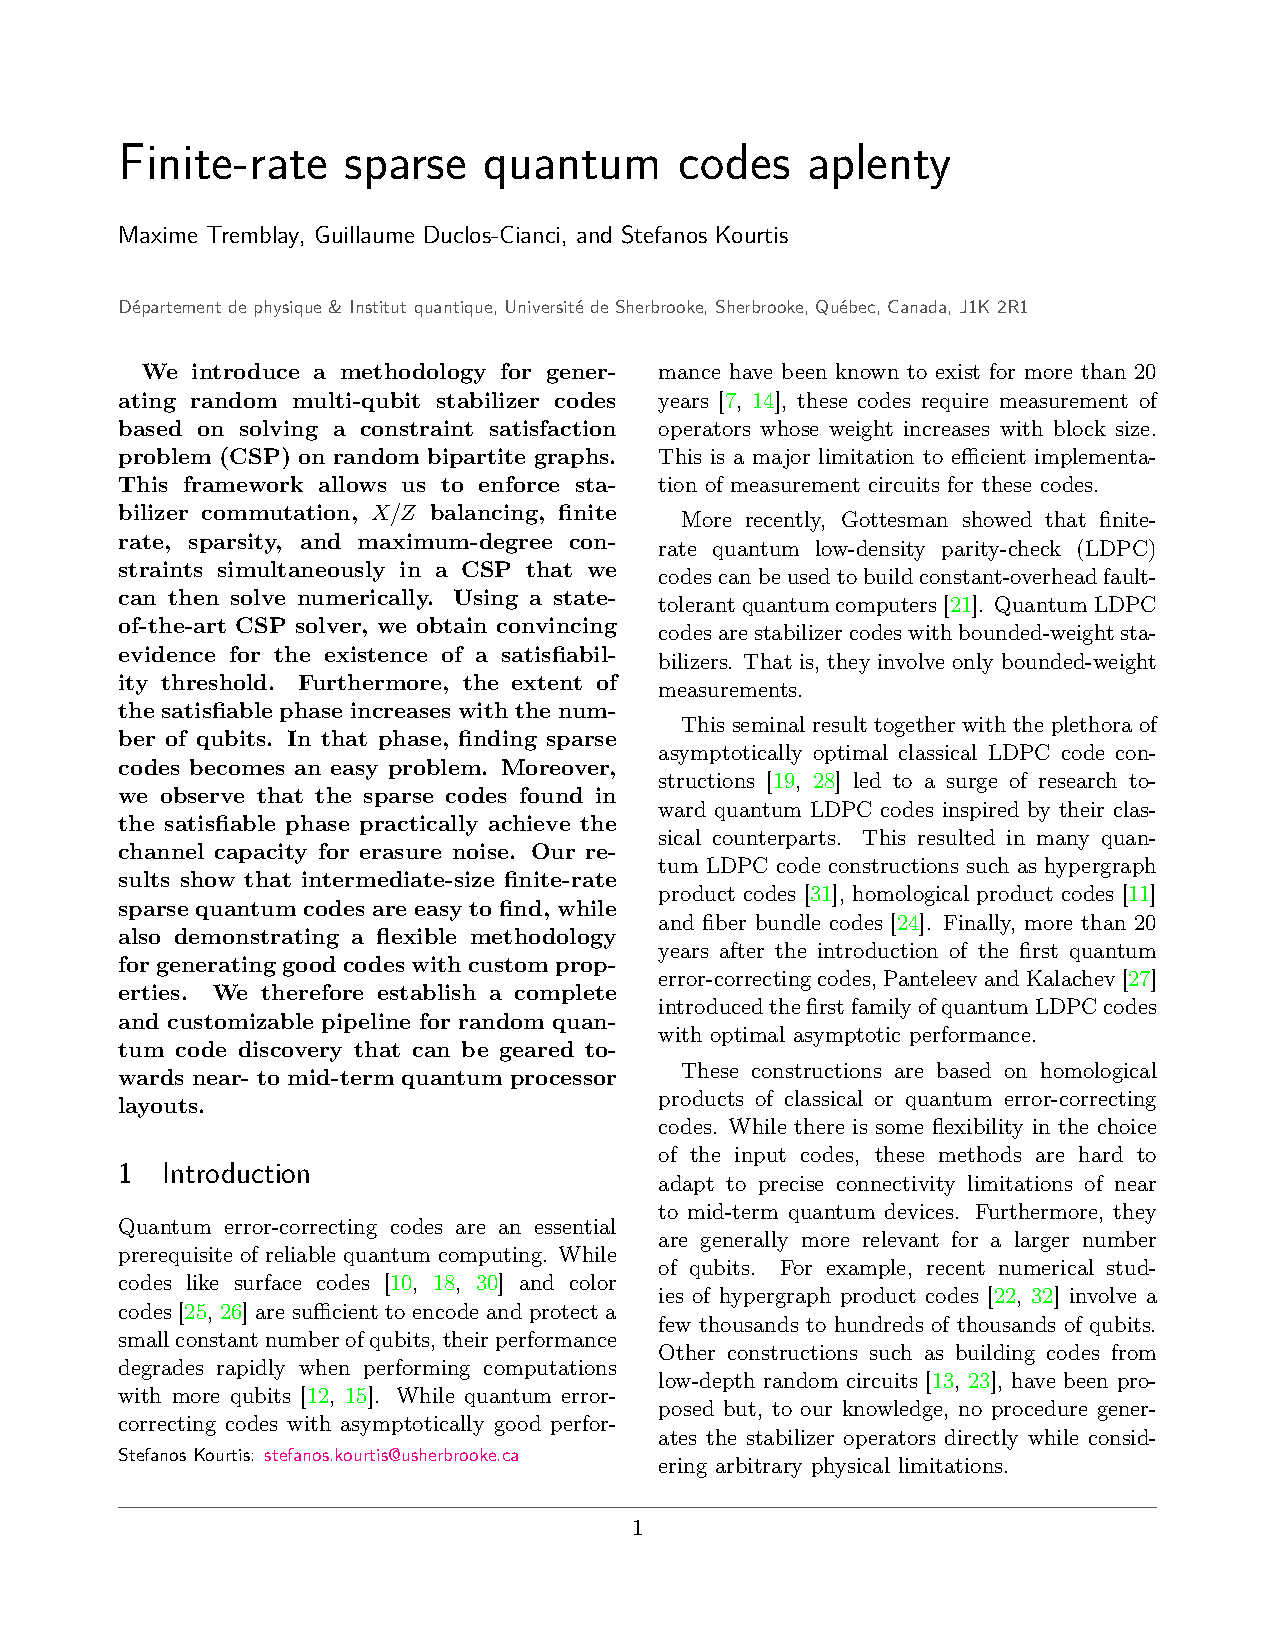
\includepdf[pages=-]{articles/sat_codes_construction.pdf}
